\question{Вторичная эмиссия из катода. Характеристики вторичной эмиссии}
Эмиссия электронов, вызываемая бомбардировкой мишени электронами, называется
\emph{вторичной}. Она обусловлена следующими процессами, происходящими в мишени:
\begin{enumerate}
    \item упругое и неупругое рассеяние первичных электронов;
    \item возбуждение внутренних вторичных электронов при взаимодействии с
    первичными электронами;
    \item каскадный процесс опбразования вторичных электронов при взаимодействии
    с другими вторичными электронами.
\end{enumerate}
Ток вторичной эмиссии связывают с током первичных электронов при помощи
коэффициента вторичной эмиссии:
\[
    I_2 = \sigma I_1.
\]
Зависимость коэффициента вторичной эмиссии от энергии налетающих электронов
приведена на рисунке.
%\begin{figure}[h]
%\begin{center}
    %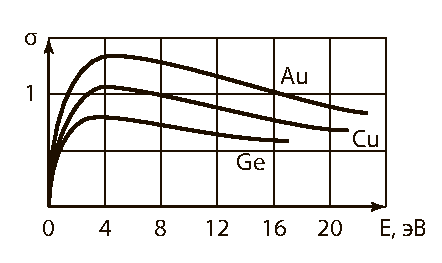
\includegraphics[width=.7\textwidth]{05_1}
%\end{center}
%\caption{Зависимость коэффициента вторичной эмиссии от энергии налетающих
         %электронов}
%\label{fig:}
%\end{figure}
\begin{table}[h]
    \center
    \begin{tabular}{|c|*{2}{>{\(}c<{\)}|}} \hline
        Вещество      & \sigma_{\max} & E_{opt},~\text{кэВ} \\ \hline
        металл        & 0.5\div0.8    & 0.2\div0.9 \\
        полупроводник & 1\div1.5      & 0.3\div0.8 \\ \hline
    \end{tabular}
\end{table}
Приведённые в таблице величины зависят от природы эмиттера, его внутренней
структуры, а также от конфигурации пучка первичных электронов.

Зависимость \( \sigma(E_1) \) для большинства веществ неплохо описывается
эмпирической формулой:
\[
    \sigma = 4\frac{E}{E_{opt}}\left(1+\frac{E}{E_{opt}}\right)^{-2}.
\]

При взаимодействии первичных электронов с мишенью большая часть вторичных
электронов образуется в конце пути, так как именно там первичный электрон
рассеивает большую часть своей энергии. Поэтому при больших энергиях он
останавливается слишком глубоко в веществе и лишь малая часть вторичных
электронов вылетает из эмиттера.

Тут что-то про угловое распределение и ещё 2 графика.

